\documentclass[12pt]{beamer}

\usepackage{slides}

\begin{document}

\begin{frame}
	\maketitle
\end{frame}

\begin{section}{Introduction}

\begin{frame}{Introduction: Types of Contact Tracing}
  \begin{itemize}
    \item Digital contact tracing (DCT)
    \item Proximity tracing
    \item Decentralized DCT
      \begin{itemize}
        \item Broadcast model
        \item Message-oriented model
      \end{itemize}
  \end{itemize}
\end{frame}

\begin{frame}{Introduction: Limitations of Other Approaches}
  \begin{itemize}
    \item No DCT approach exists that incorporates both non-diagnostic information and indirect contacts to estimate infection risk.
    \item Account for indirect contact can substantially improve the efficacy of DCT \citep{PozoMartin2023}.
    \item \citet{Cherini2023} propose exchanging pseudonyms of indirect contacts, but restrict themselves to diagnostic testing.
    \item \citet{Gupta2023} incorporate non-diagnostic information, but do not account for indirect contact.
  \end{itemize}
\end{frame}

\begin{frame}{Introduction: ShareTrace}
  \begin{itemize}
    \item Accounts for both non-diagnostic information and indirect contact to estimate infection risk.
    \item First proposed by \citet{Ayday2020, Ayday2021} as part of a collaboration with Dataswyft.
    \item \citet{Ayday2021} 
  \end{itemize}
\end{frame}
\end{section}

\begin{section}{Proposed Design}

\begin{frame}{Proposed Design}
  
\end{frame}

\end{section}

\begin{section}{Evaluation}

\begin{frame}[allowframebreaks]{Experiment 1: Accuracy}
  \begin{figure}
    \centering
    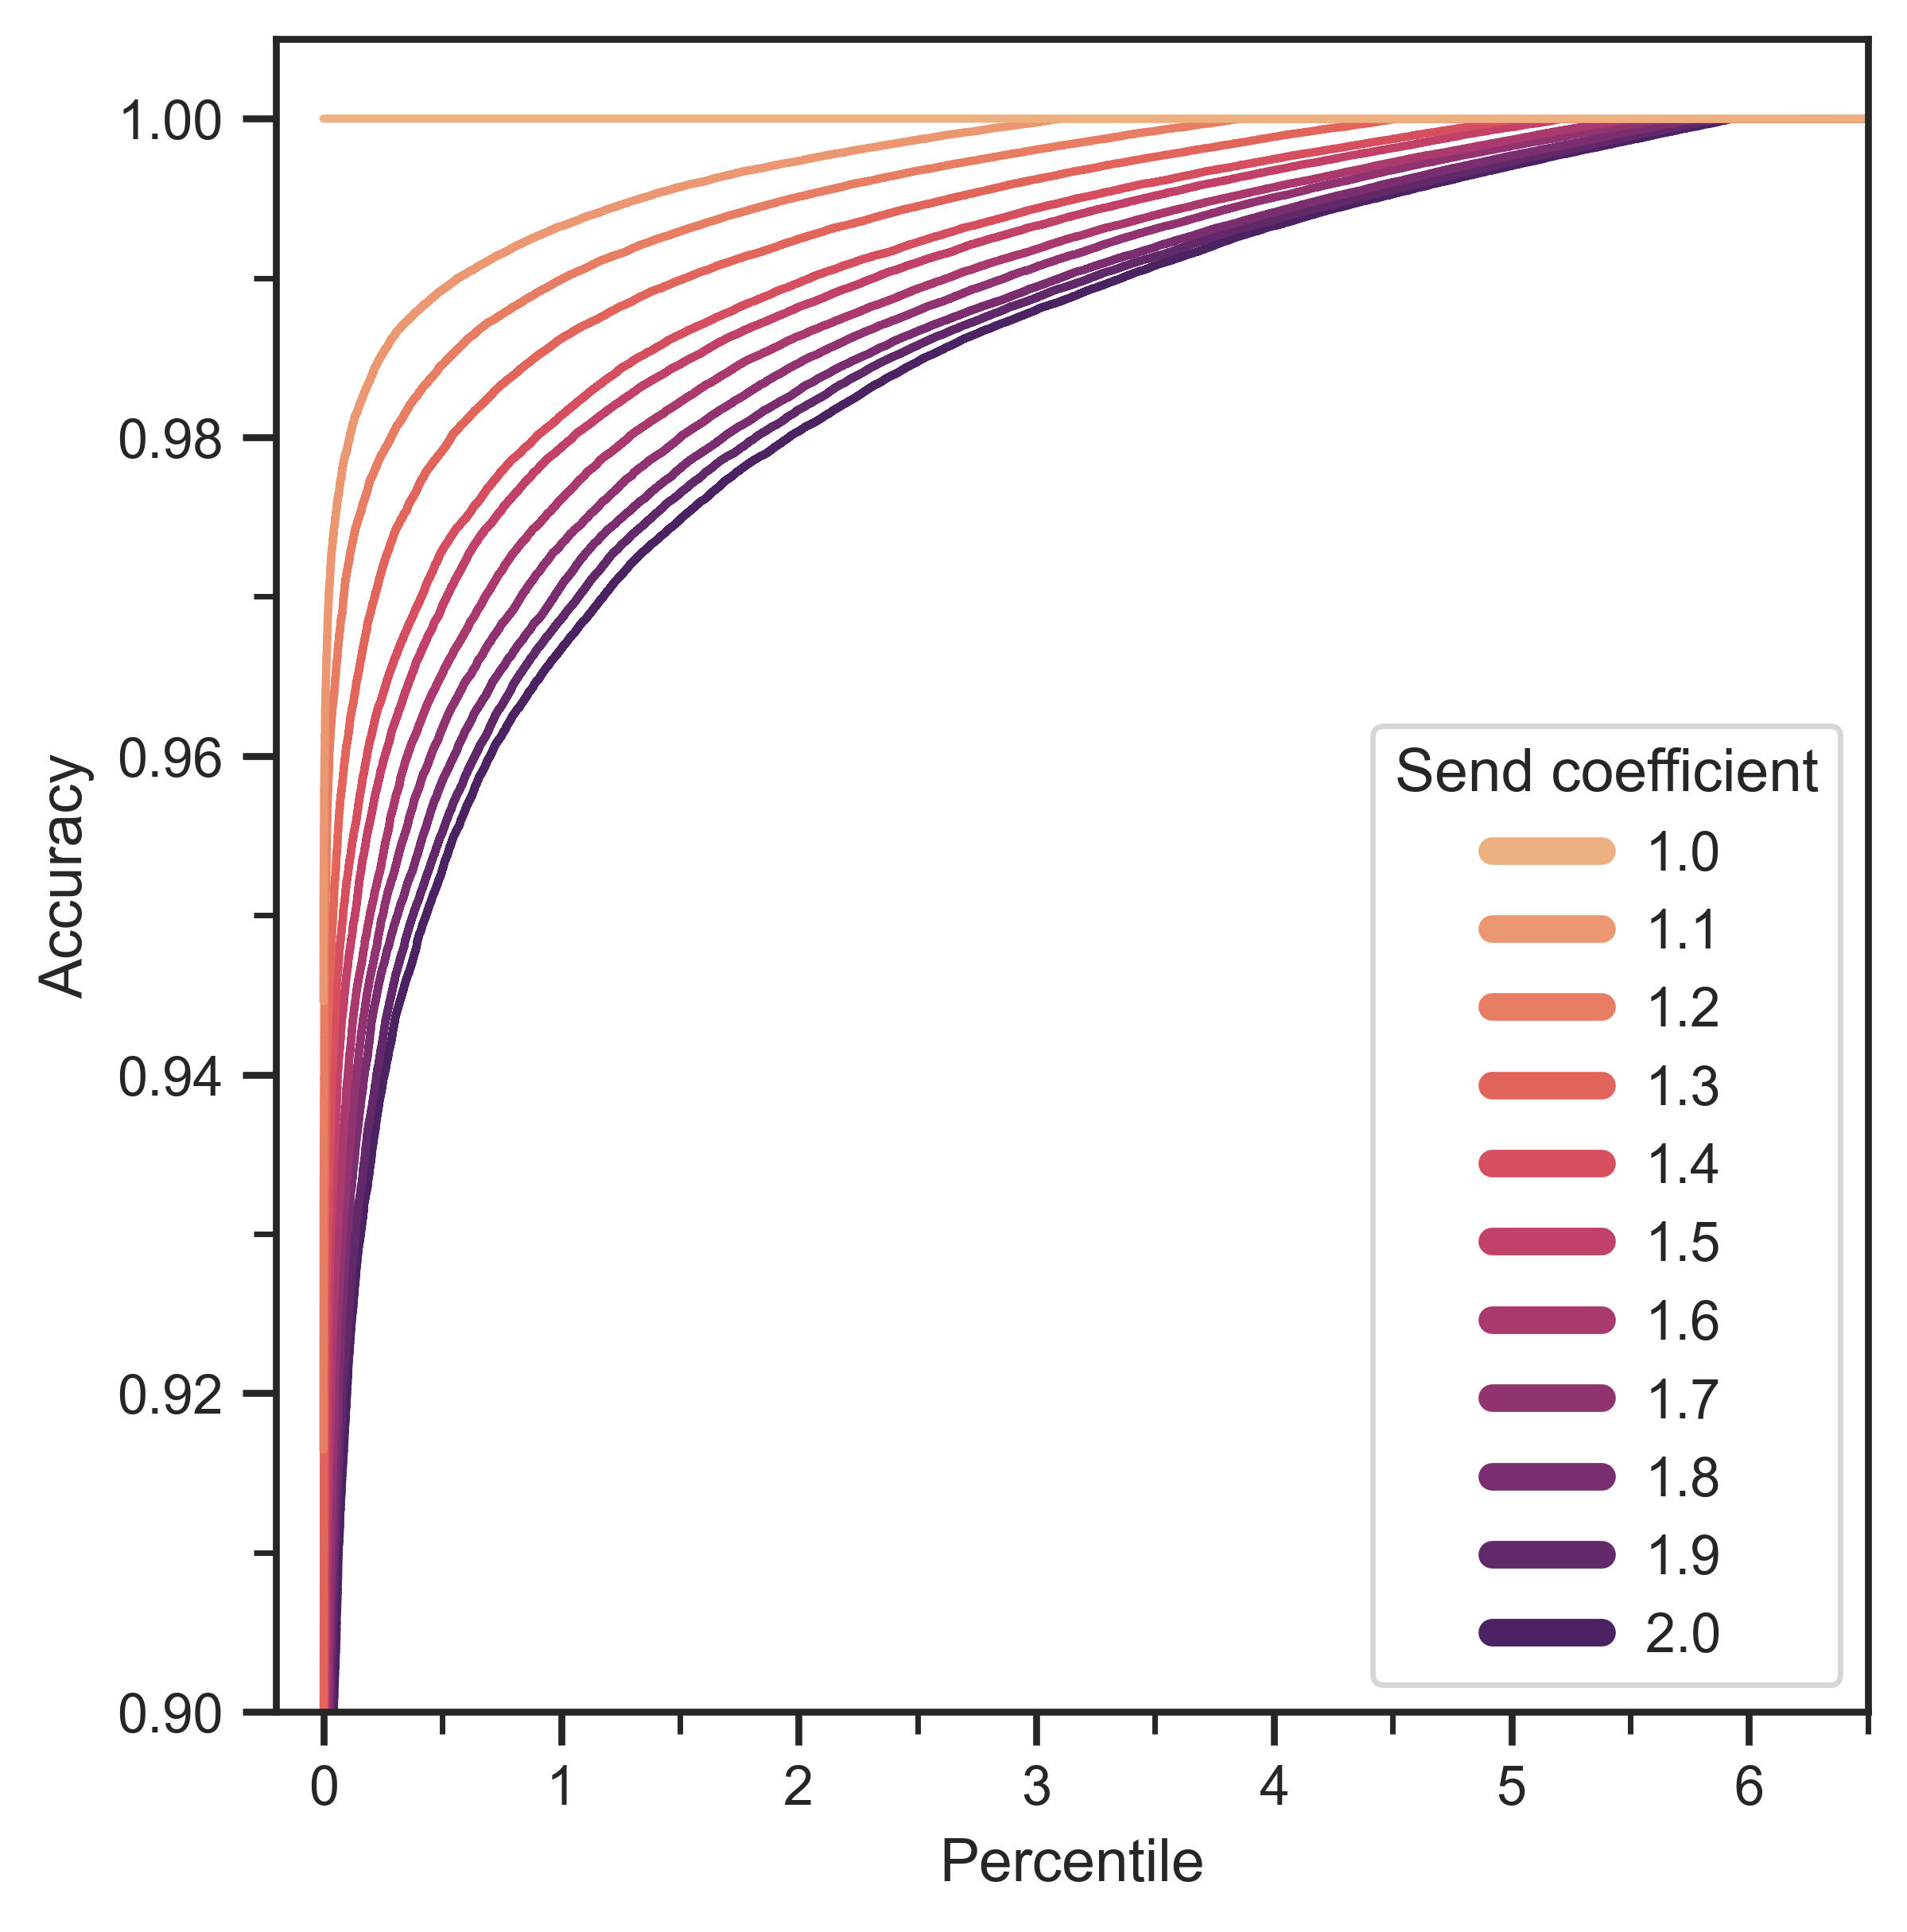
\includegraphics[height=\squareFigHeight]{accuracy-percentiles}
    \caption[Cumulative accuracy distributions]{Cumulative accuracy distributions.}
  \end{figure}

  \begin{figure}
    \centering
    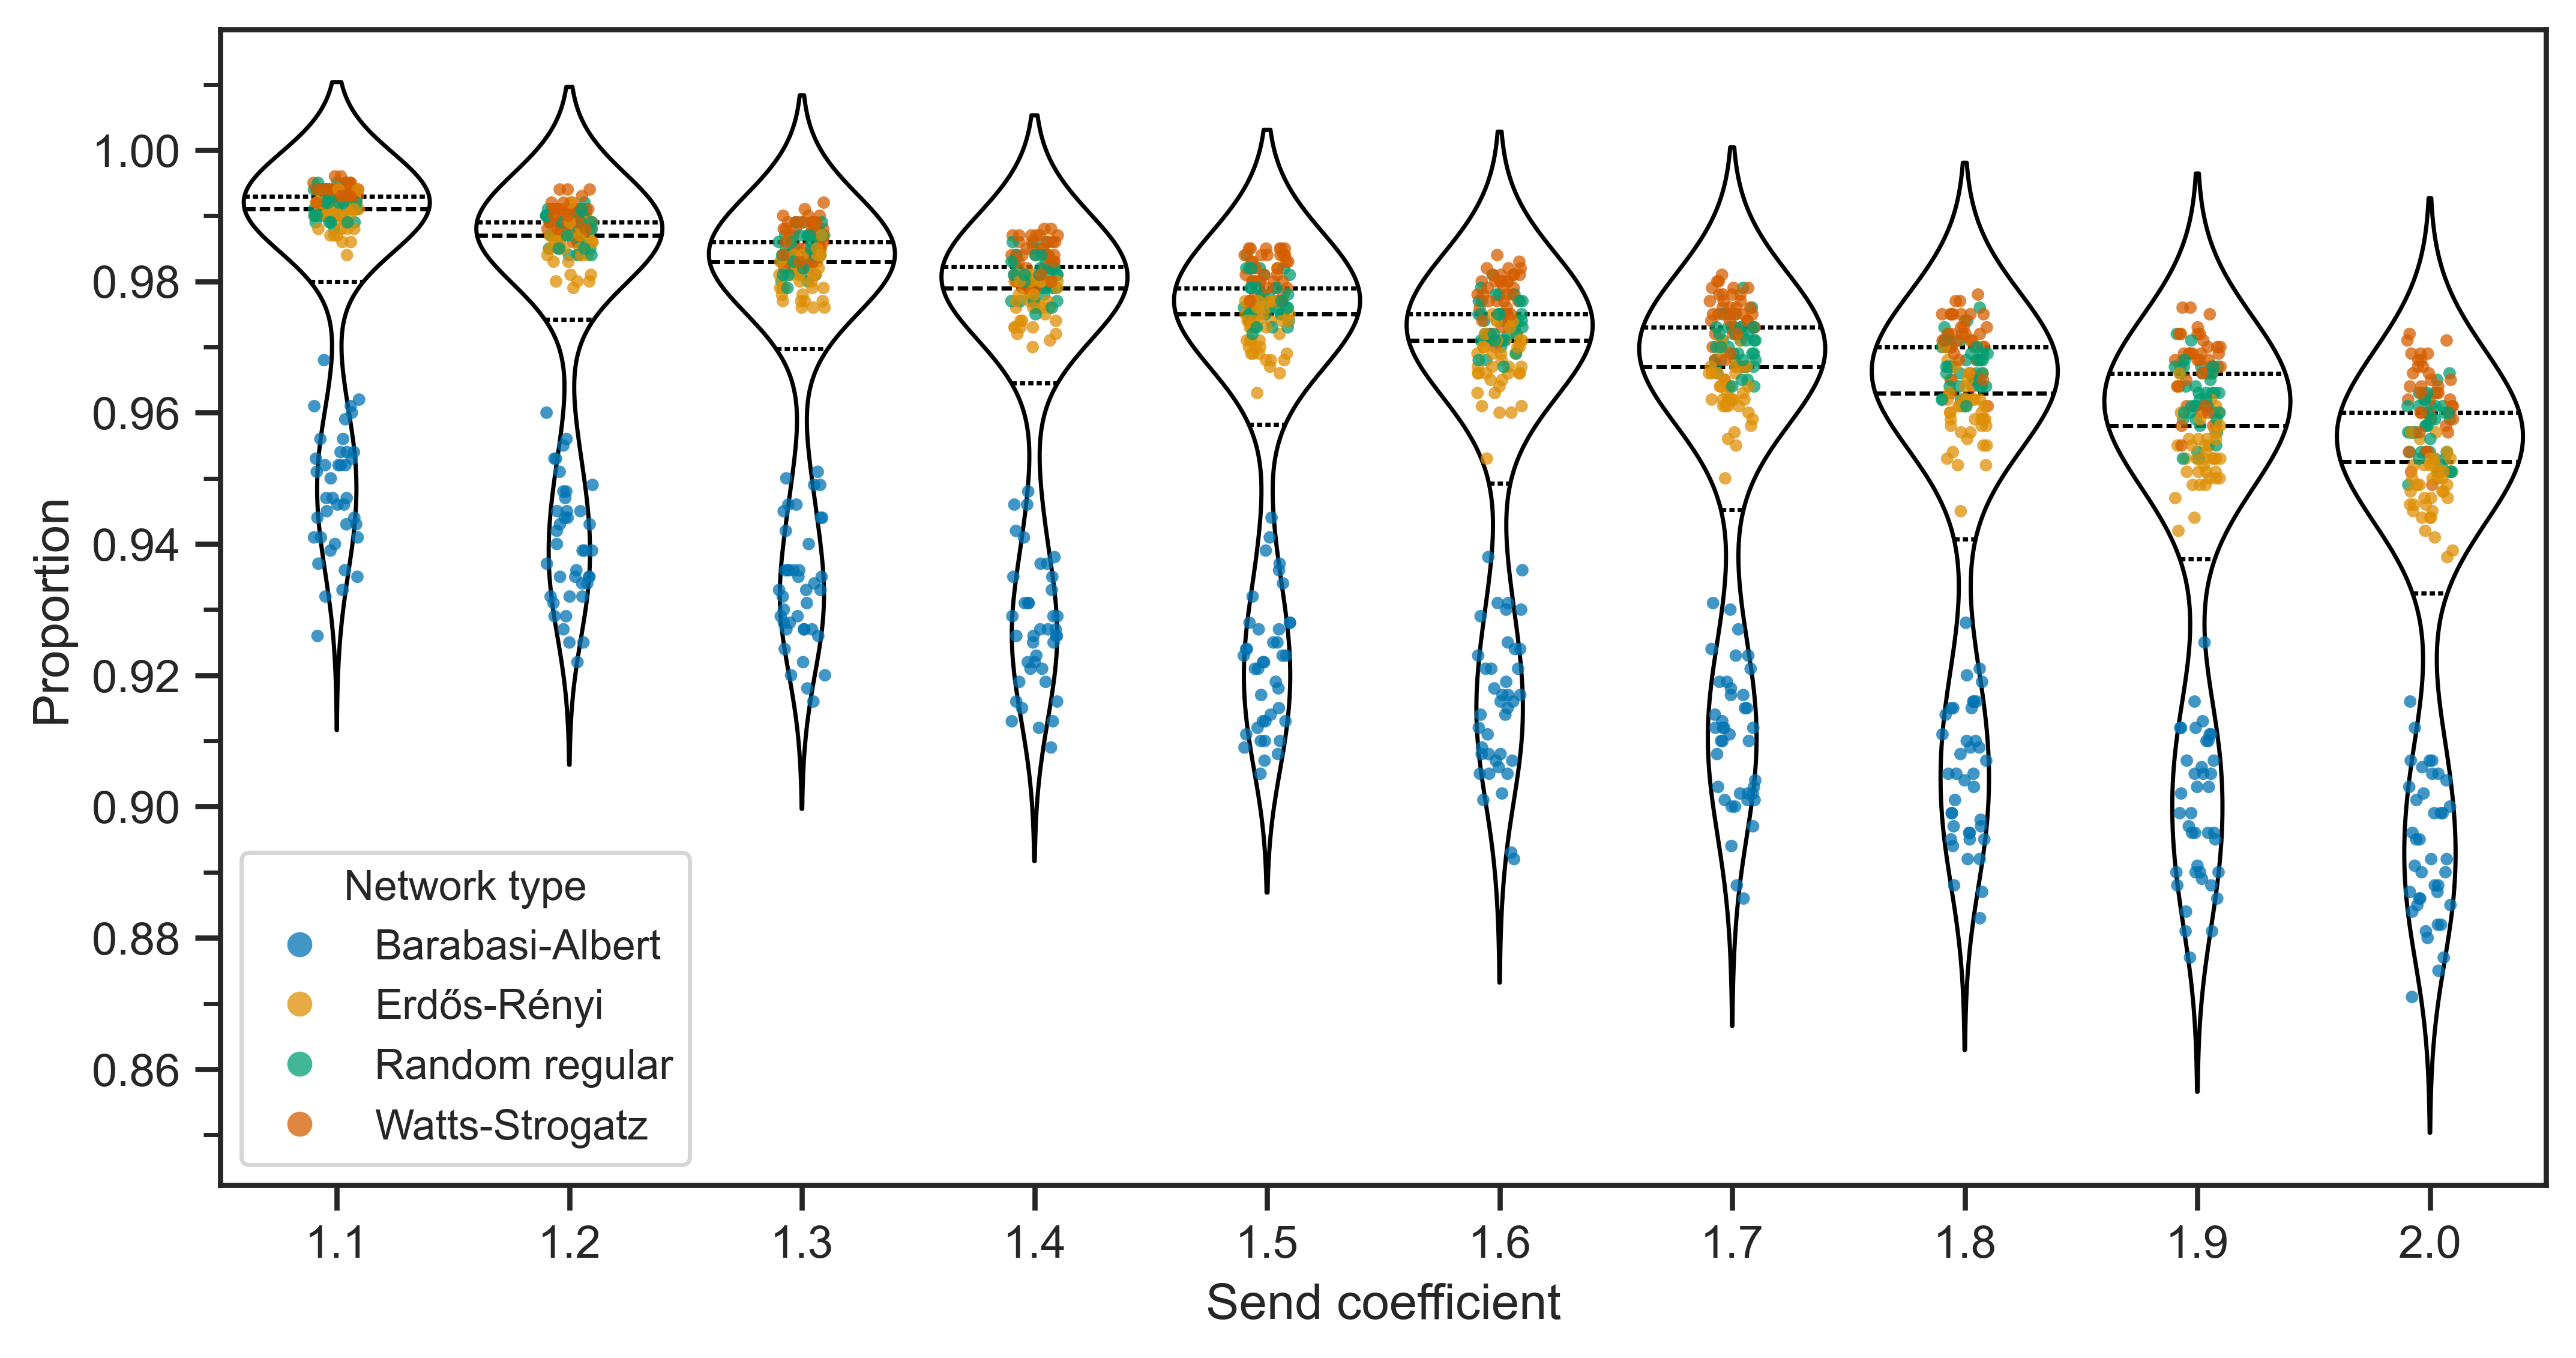
\includegraphics[width=\wideFigWidth]{accuracy-proportions}
    \caption[Send coefficient optimality distributions]{Send coefficient optimality distributions. The dashed line inside each violin marks the median. The upper and lower dotted lines inside each violin mark the upper and lower quartiles, respectively.}
  \end{figure}
\end{frame}

\begin{frame}[allowframebreaks]{Experiment 1: Efficiency}
  \begin{figure}
    \centering
    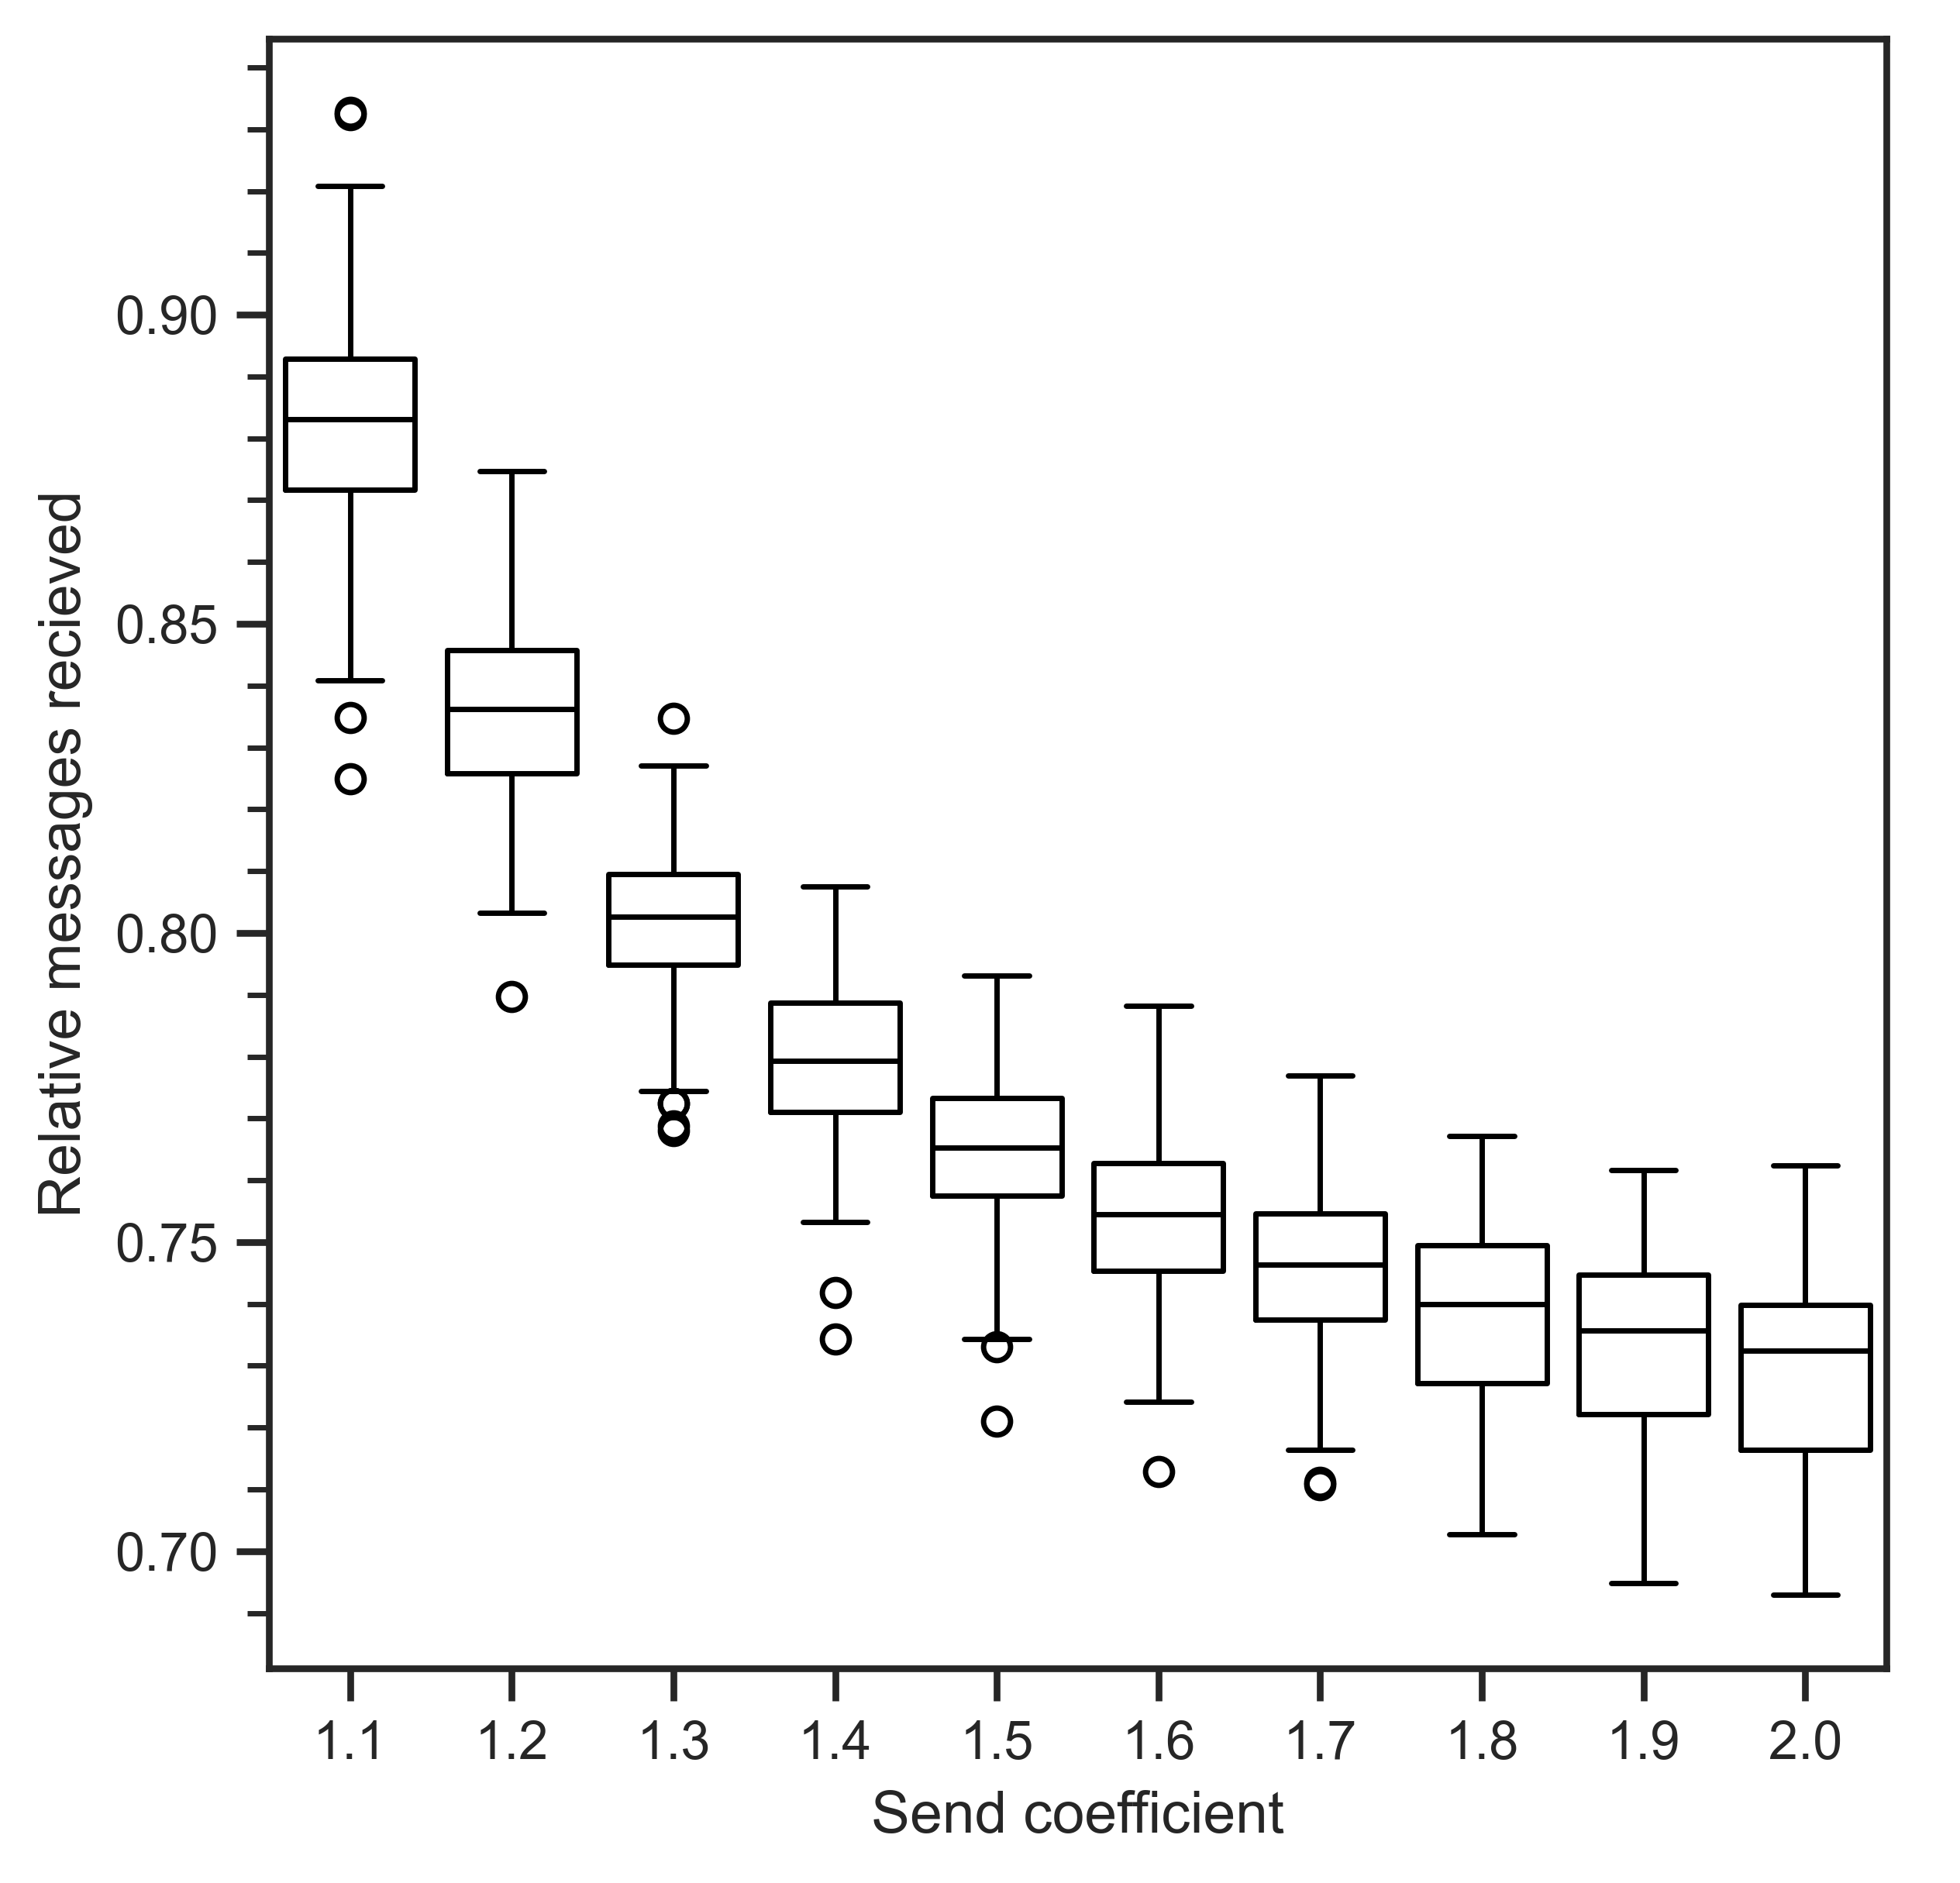
\includegraphics[height=\squareFigHeight]{relative-receives}
    \caption[Message-passing efficiency]{Message-passing efficiency. The send coefficient $\pSendCoefficient = 1$ was used as a baseline for message-passing efficiency since it was found to be the maximum send coefficient that achieves perfect accuracy.}
  \end{figure}

  \begin{figure}
    \centering
    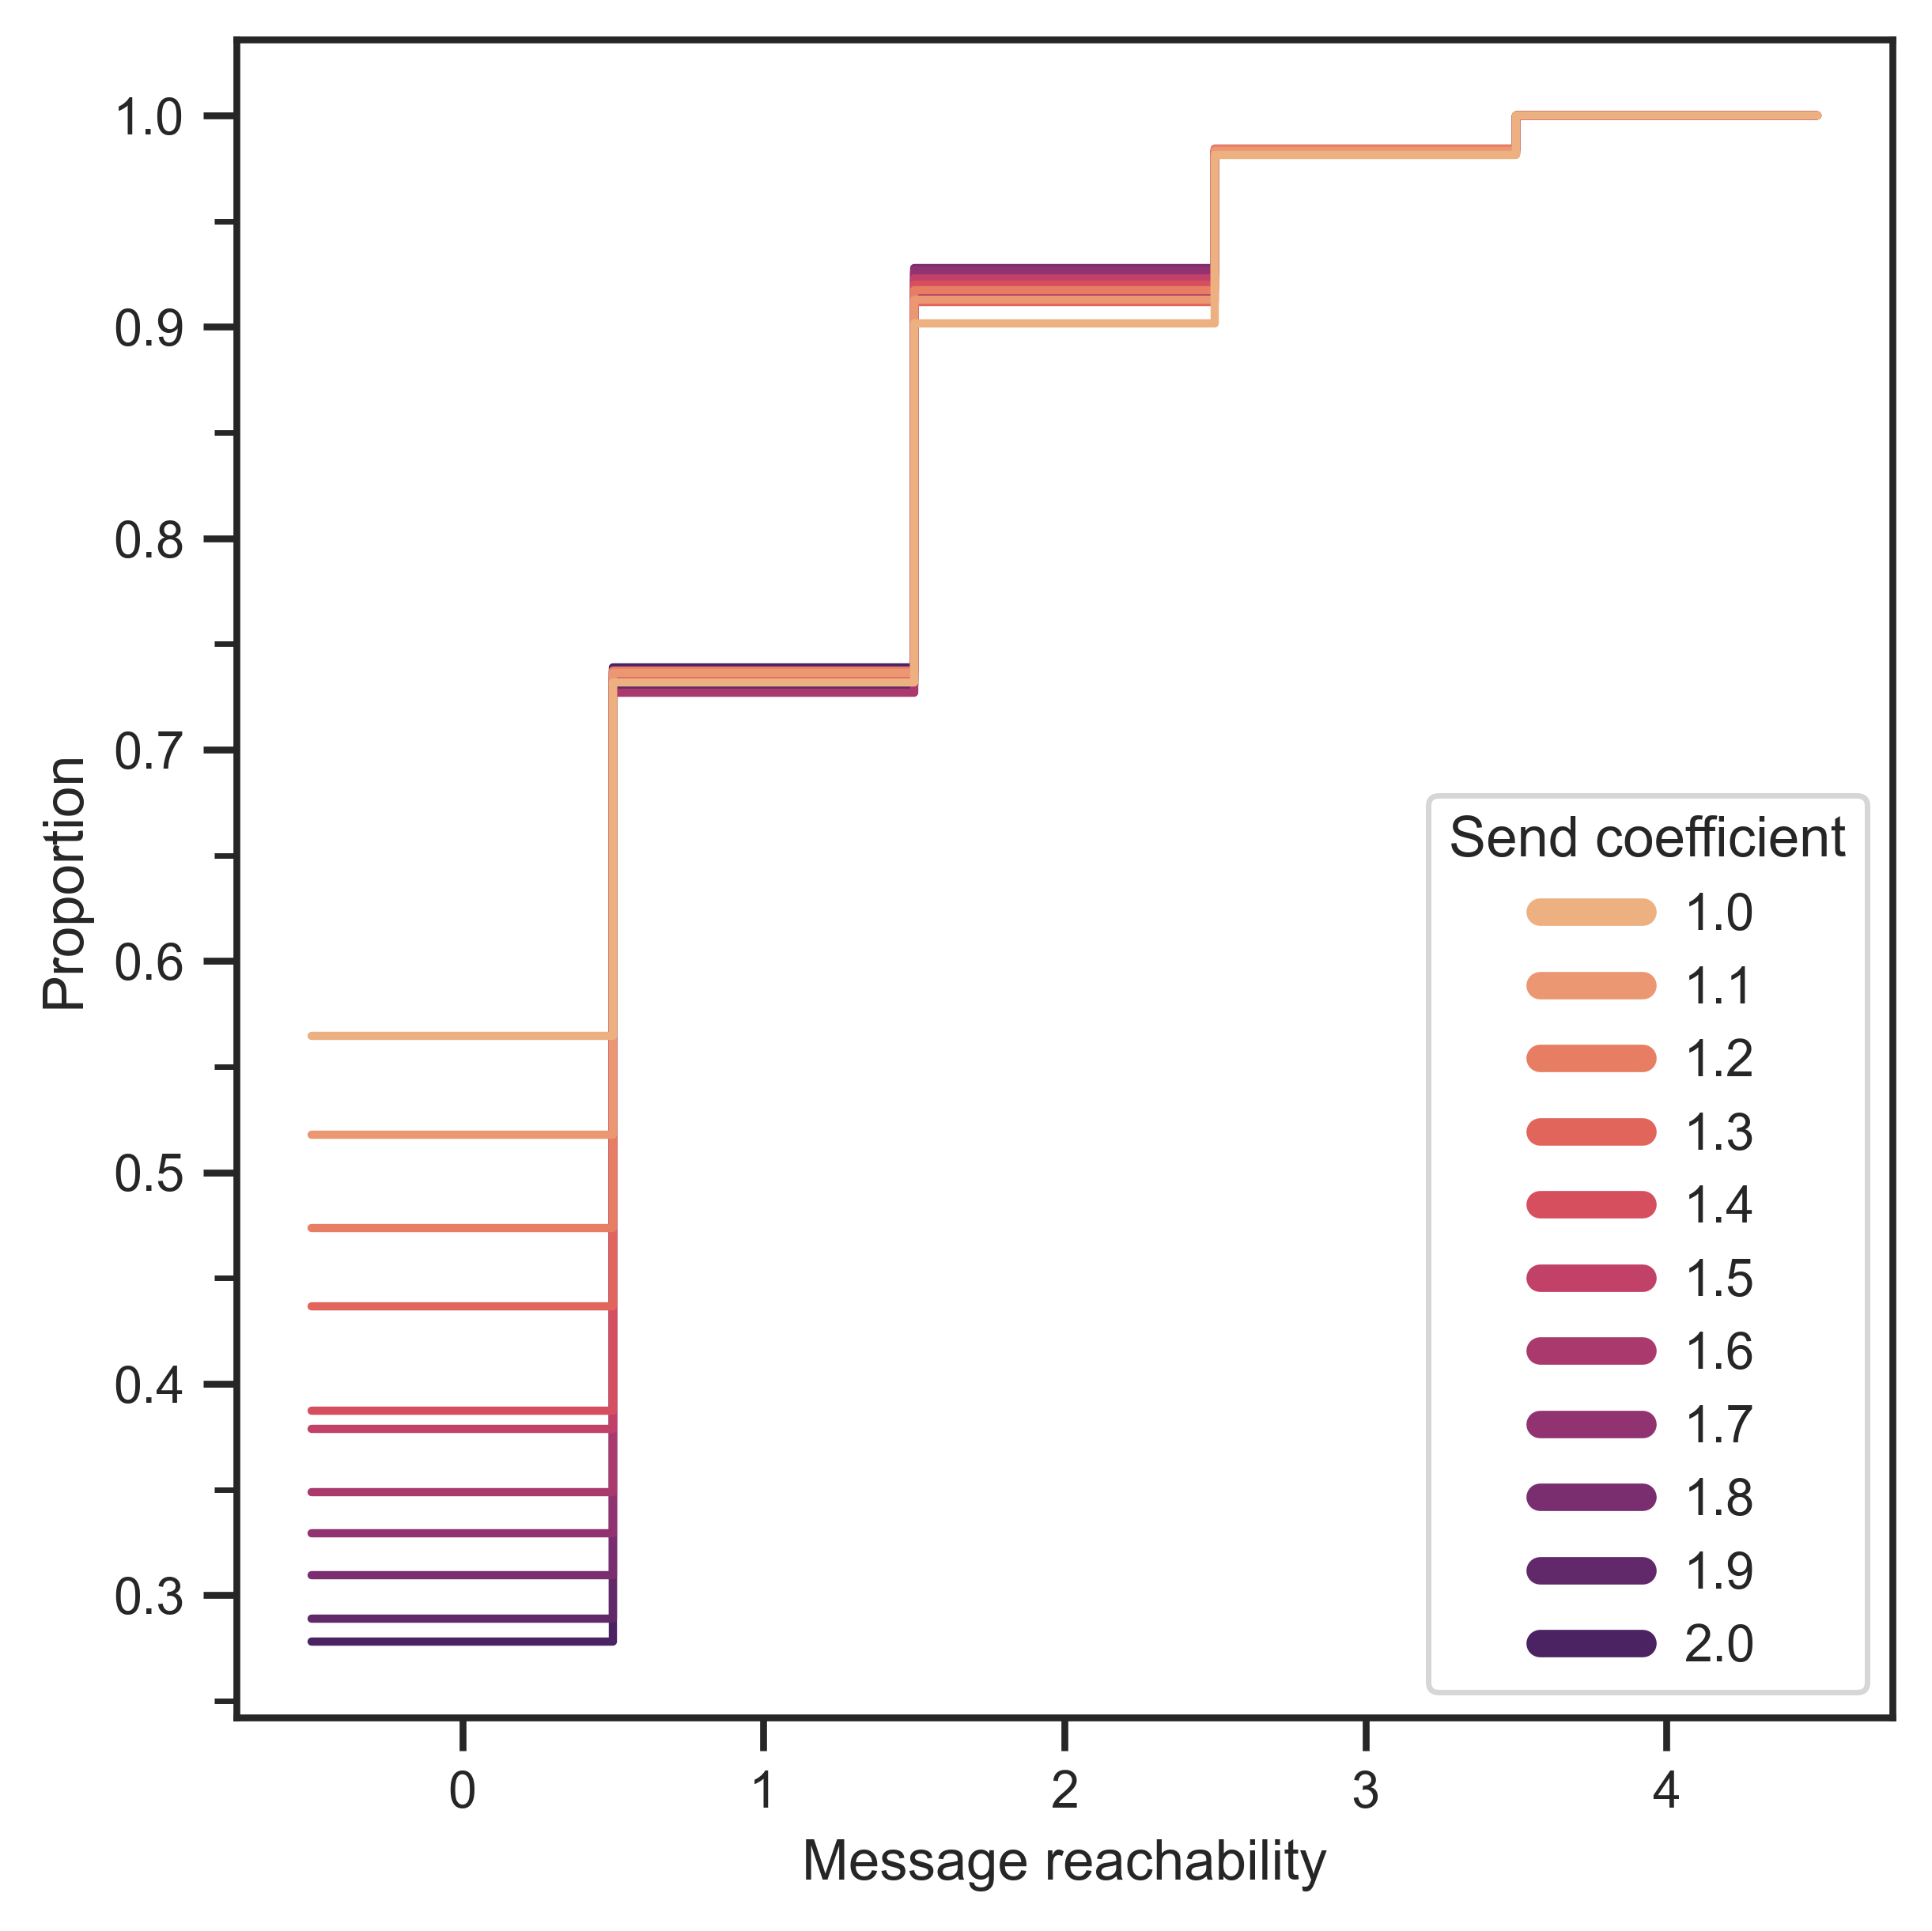
\includegraphics[height=\squareFigHeight]{message-reachability}
    \caption[Message reachability cumulative distributions]{Message reachability cumulative distributions.}
  \end{figure}
\end{frame}

\begin{frame}[allowframebreaks]{Experiment 1: Exploration}
  \begin{figure}
    \centering
    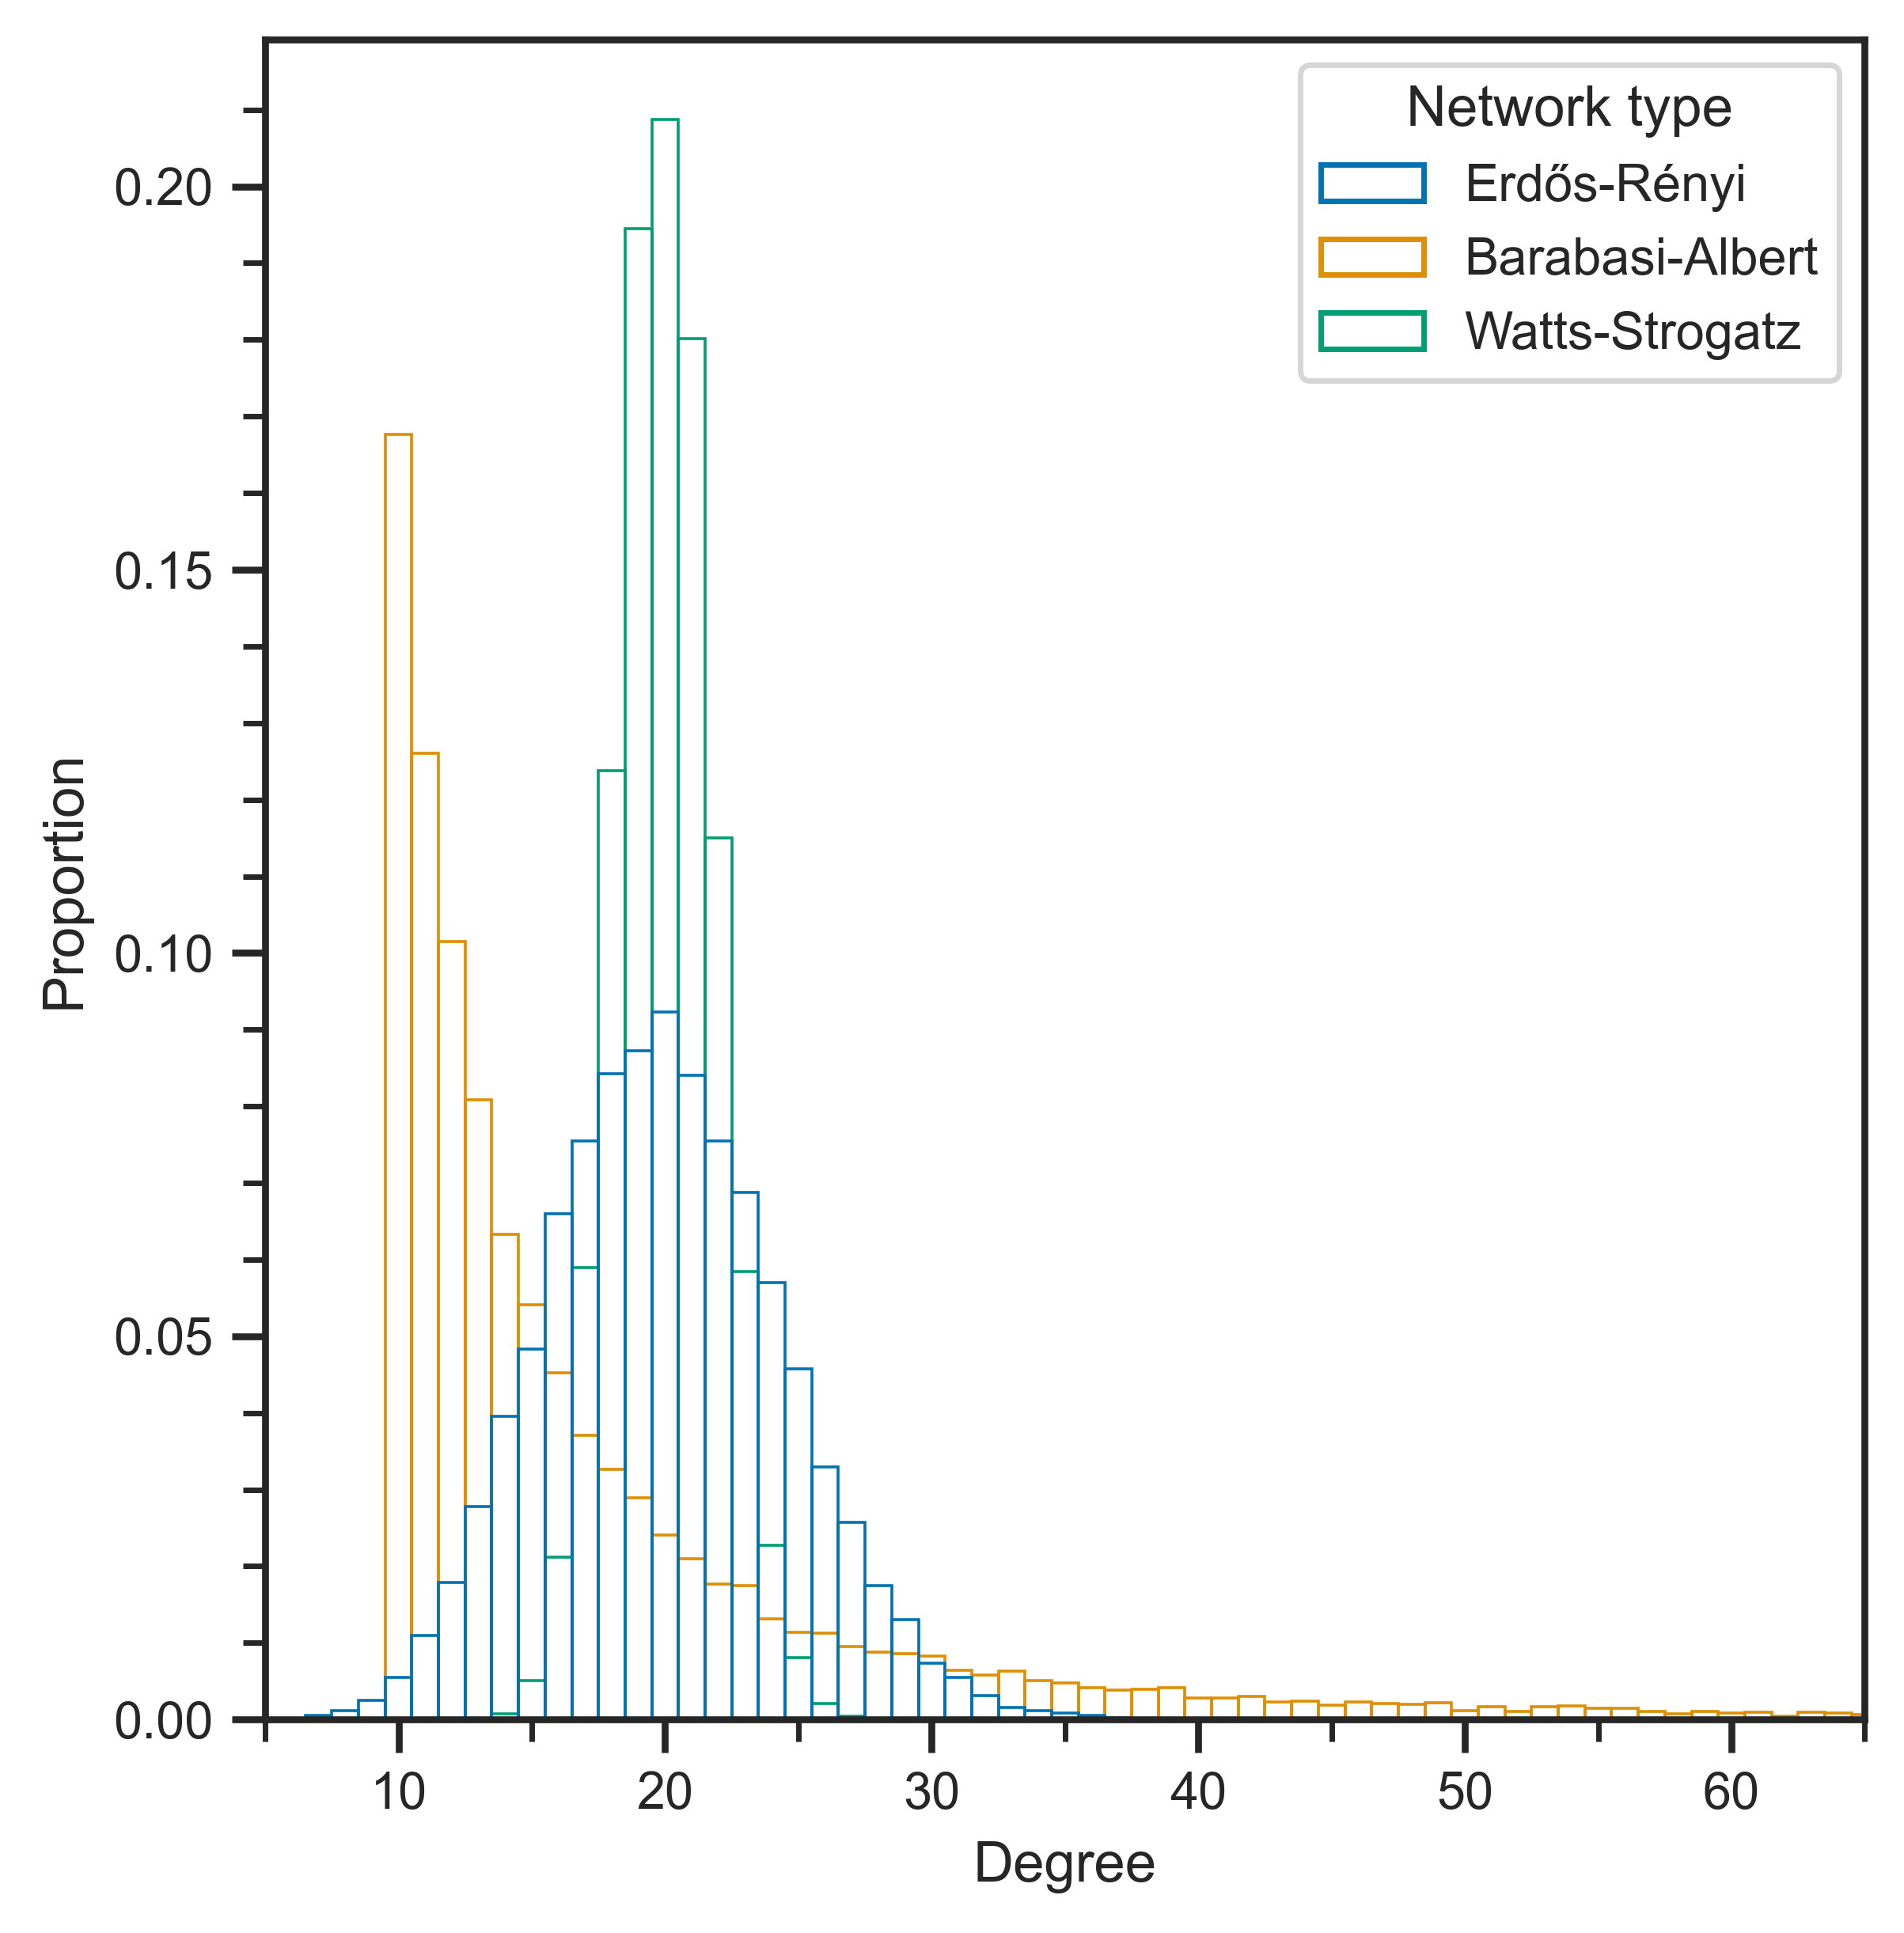
\includegraphics[height=\squareFigHeight]{network-degree-distributions}
    \caption[Contact network degree distributions]{Contact network degree distributions. All vertices in random regular contact networks had a degree of 20, so the distribution was omitted to provide more visual space for the distributions of other contact networks.}
  \end{figure}
  
  \begin{figure}
    \centering
    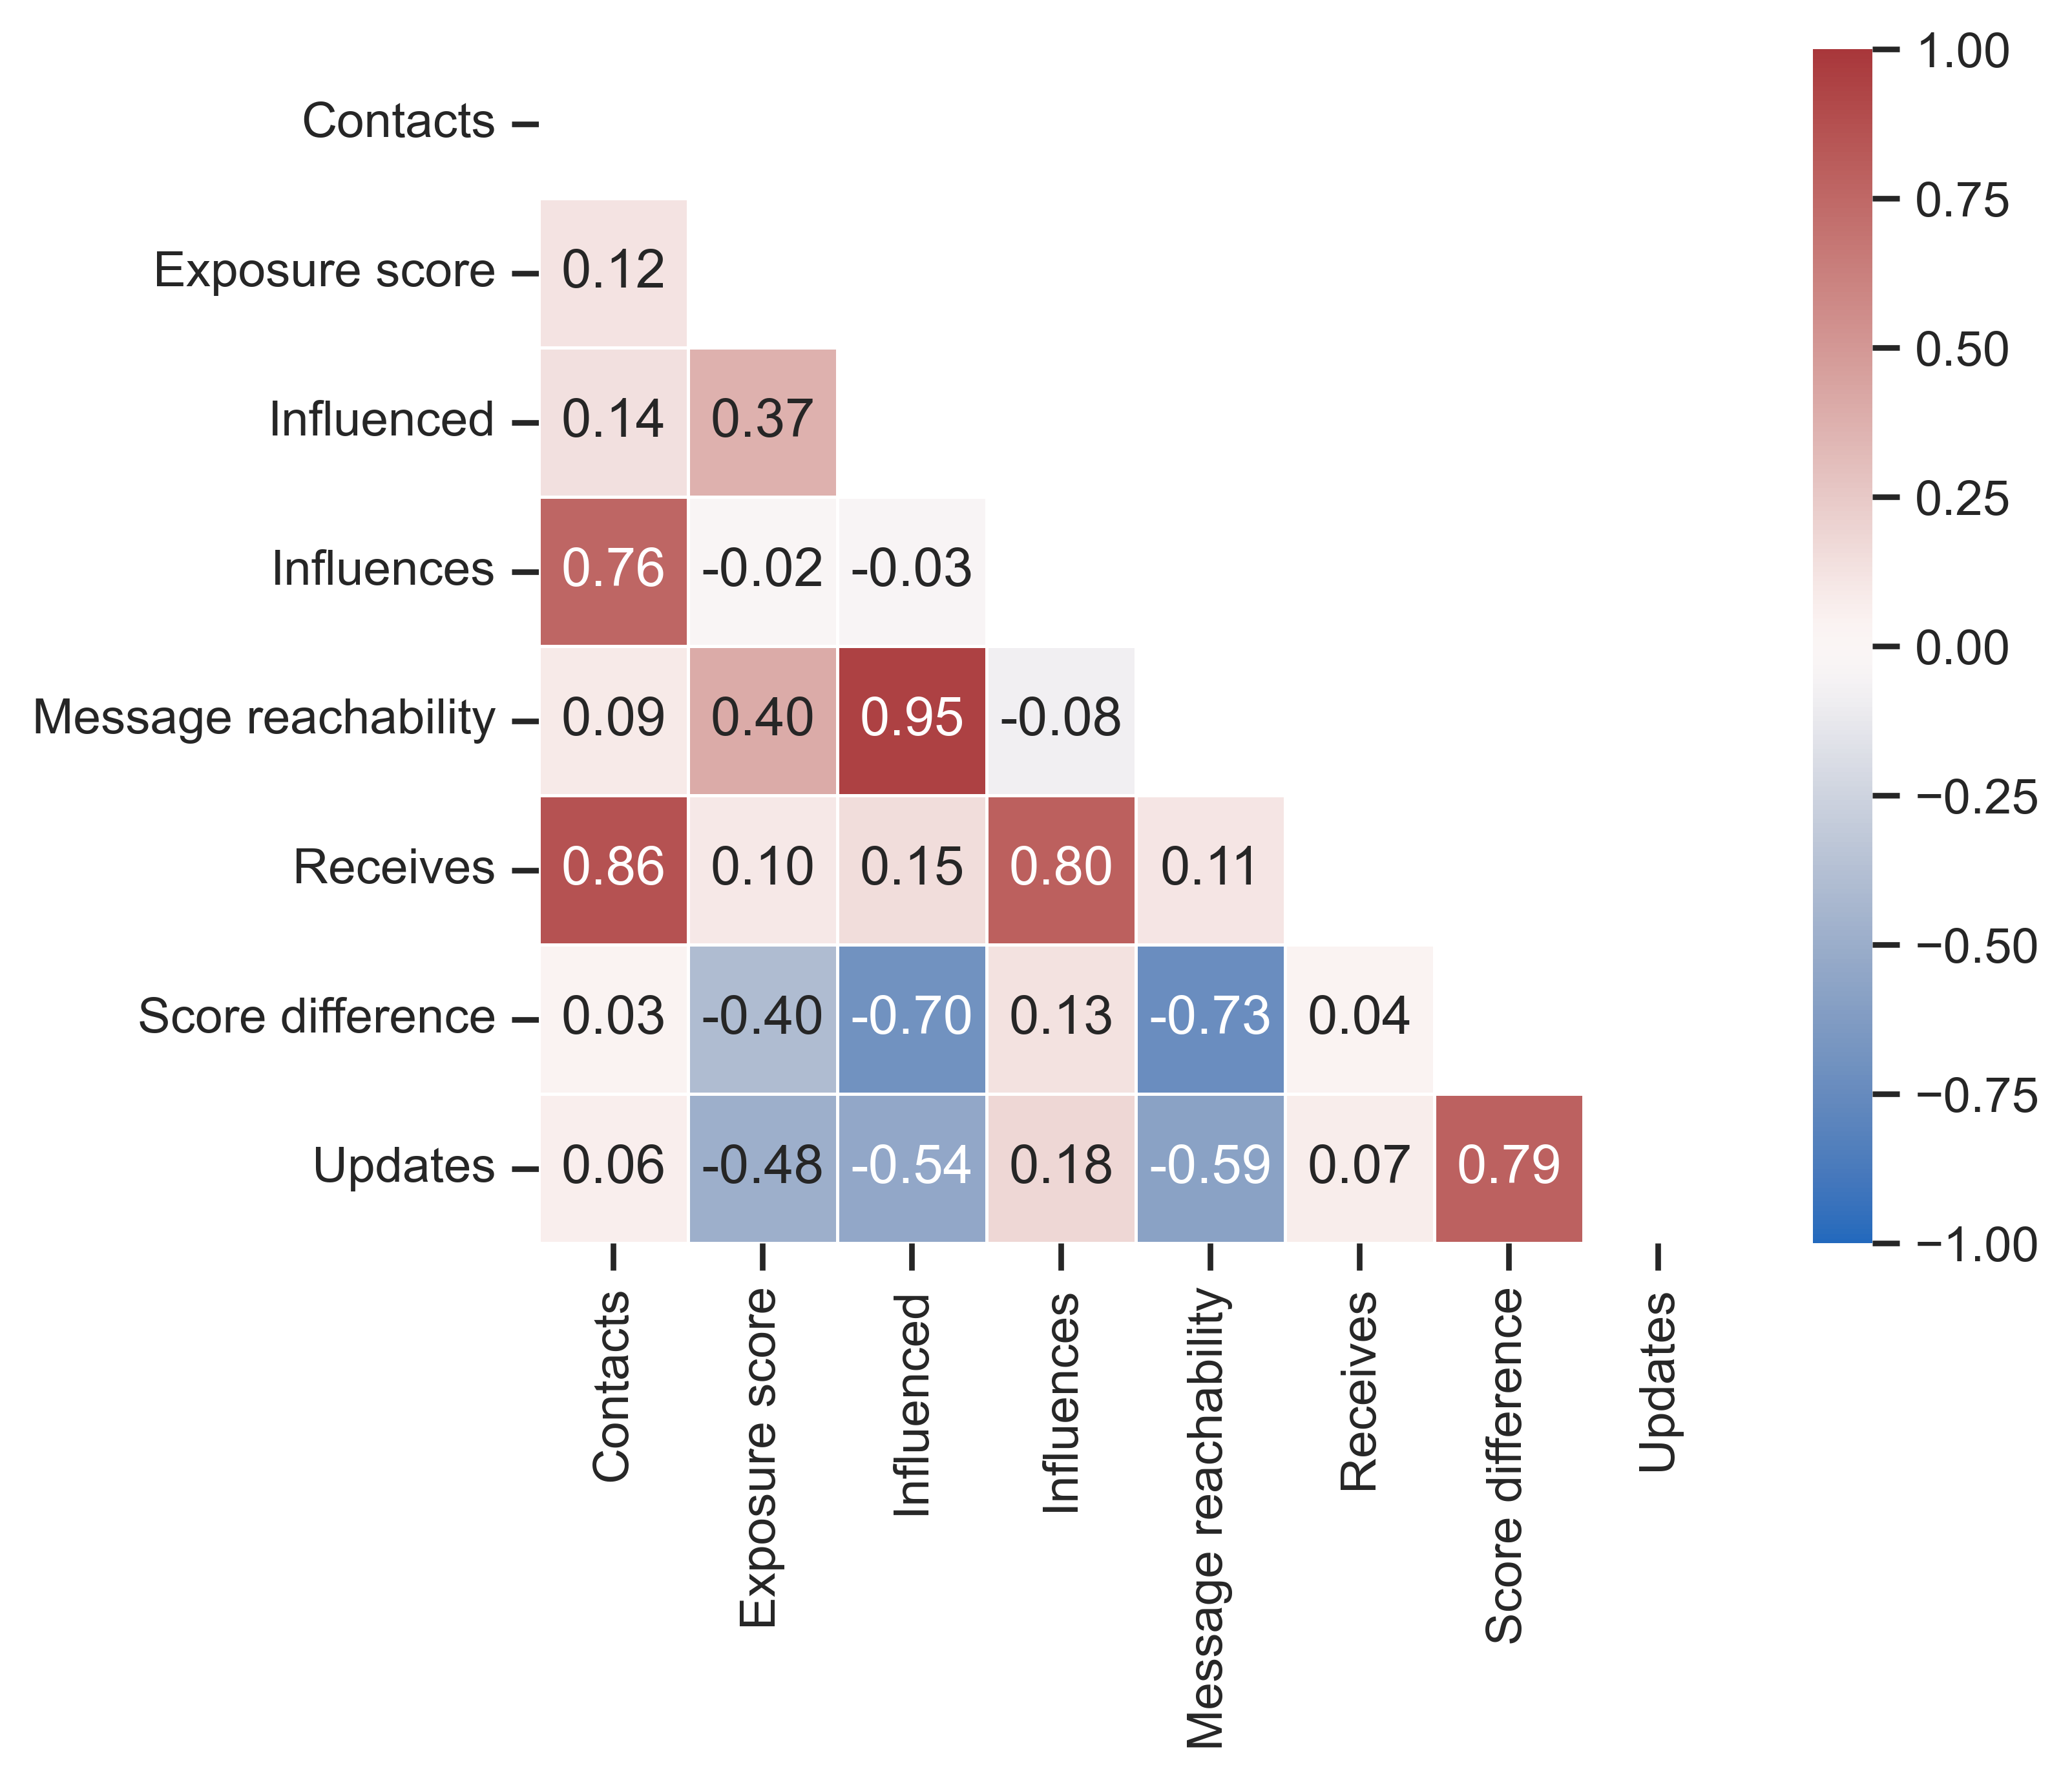
\includegraphics[height=\squareFigHeight]{correlation}
    \caption[Correlation matrix of dataset attributes]{Correlation matrix of dataset attributes. Each cell is the Spearman rank partial correlation coefficient \citep{Spearman1904}, controlling for the effect of the send coefficient. All coefficients are significant ($p < 0.01$), adjusting for multiple comparisons via the Holm–Bonferroni method \citep{Holm1979}.}
  \end{figure}
\end{frame}

\begin{frame}{Experiment 2: Benchmarking Hypothesis Testing}
\end{frame}

\begin{frame}[allowframebreaks]{Experiment 3: Benchmarking}
  \begin{figure}
    \centering
    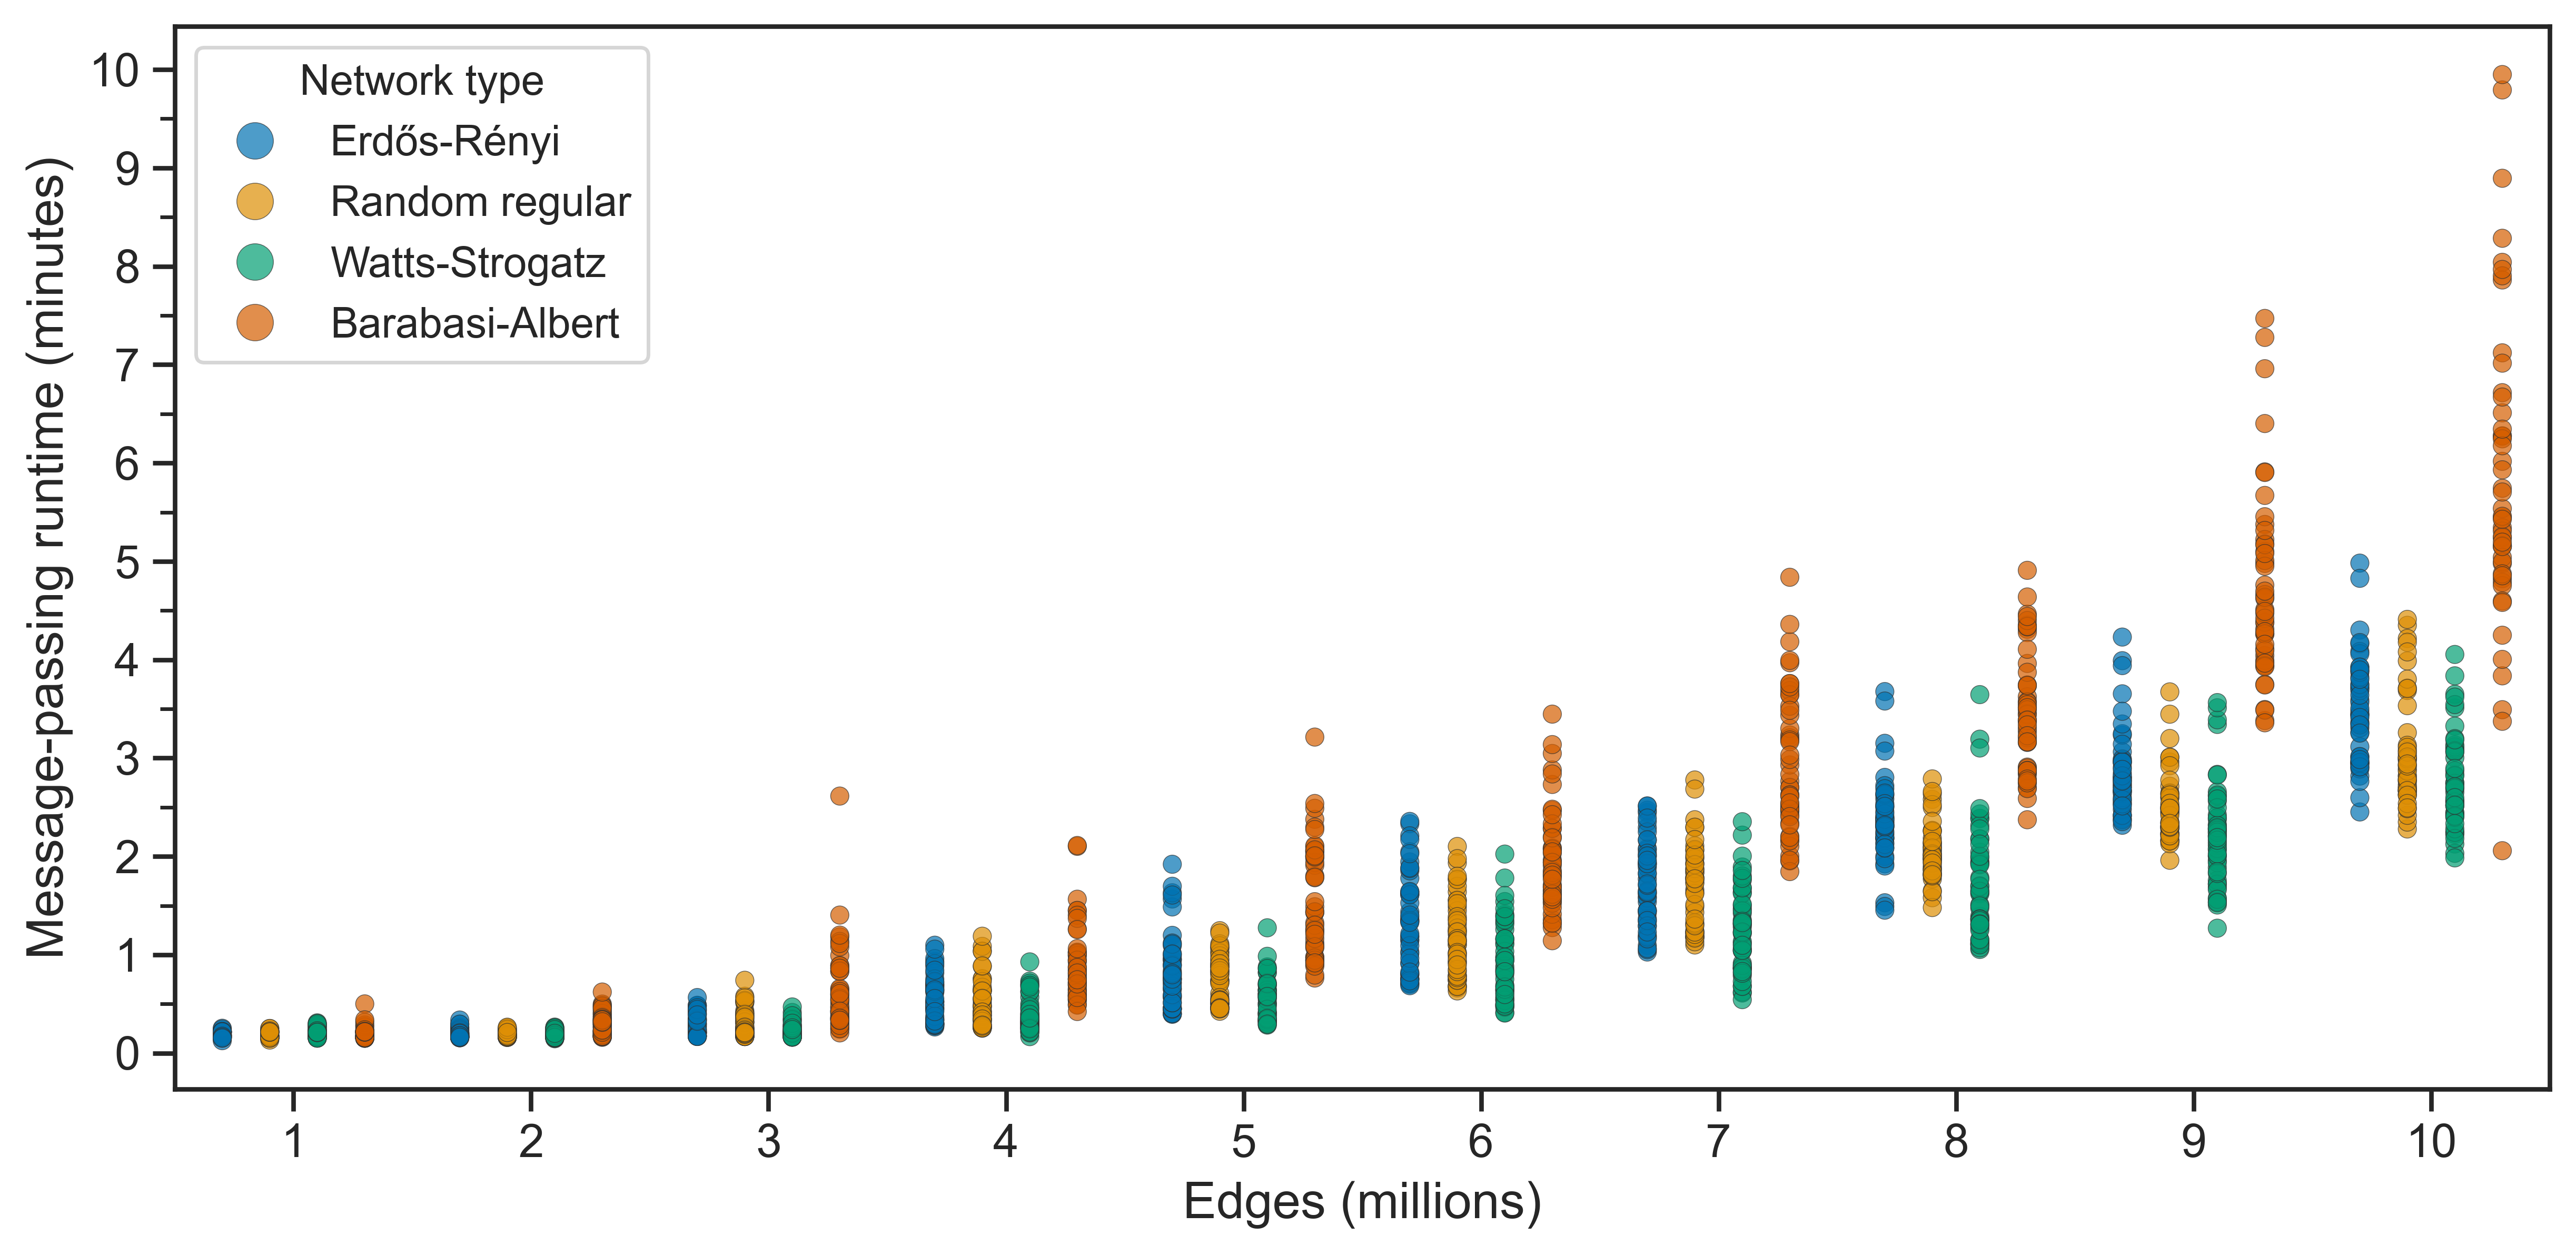
\includegraphics[width=\wideFigWidth]{runtimes}
    \caption[Message-passing runtimes]{Message-passing runtimes.}
  \end{figure}
  
  \begin{figure}
  \centering
  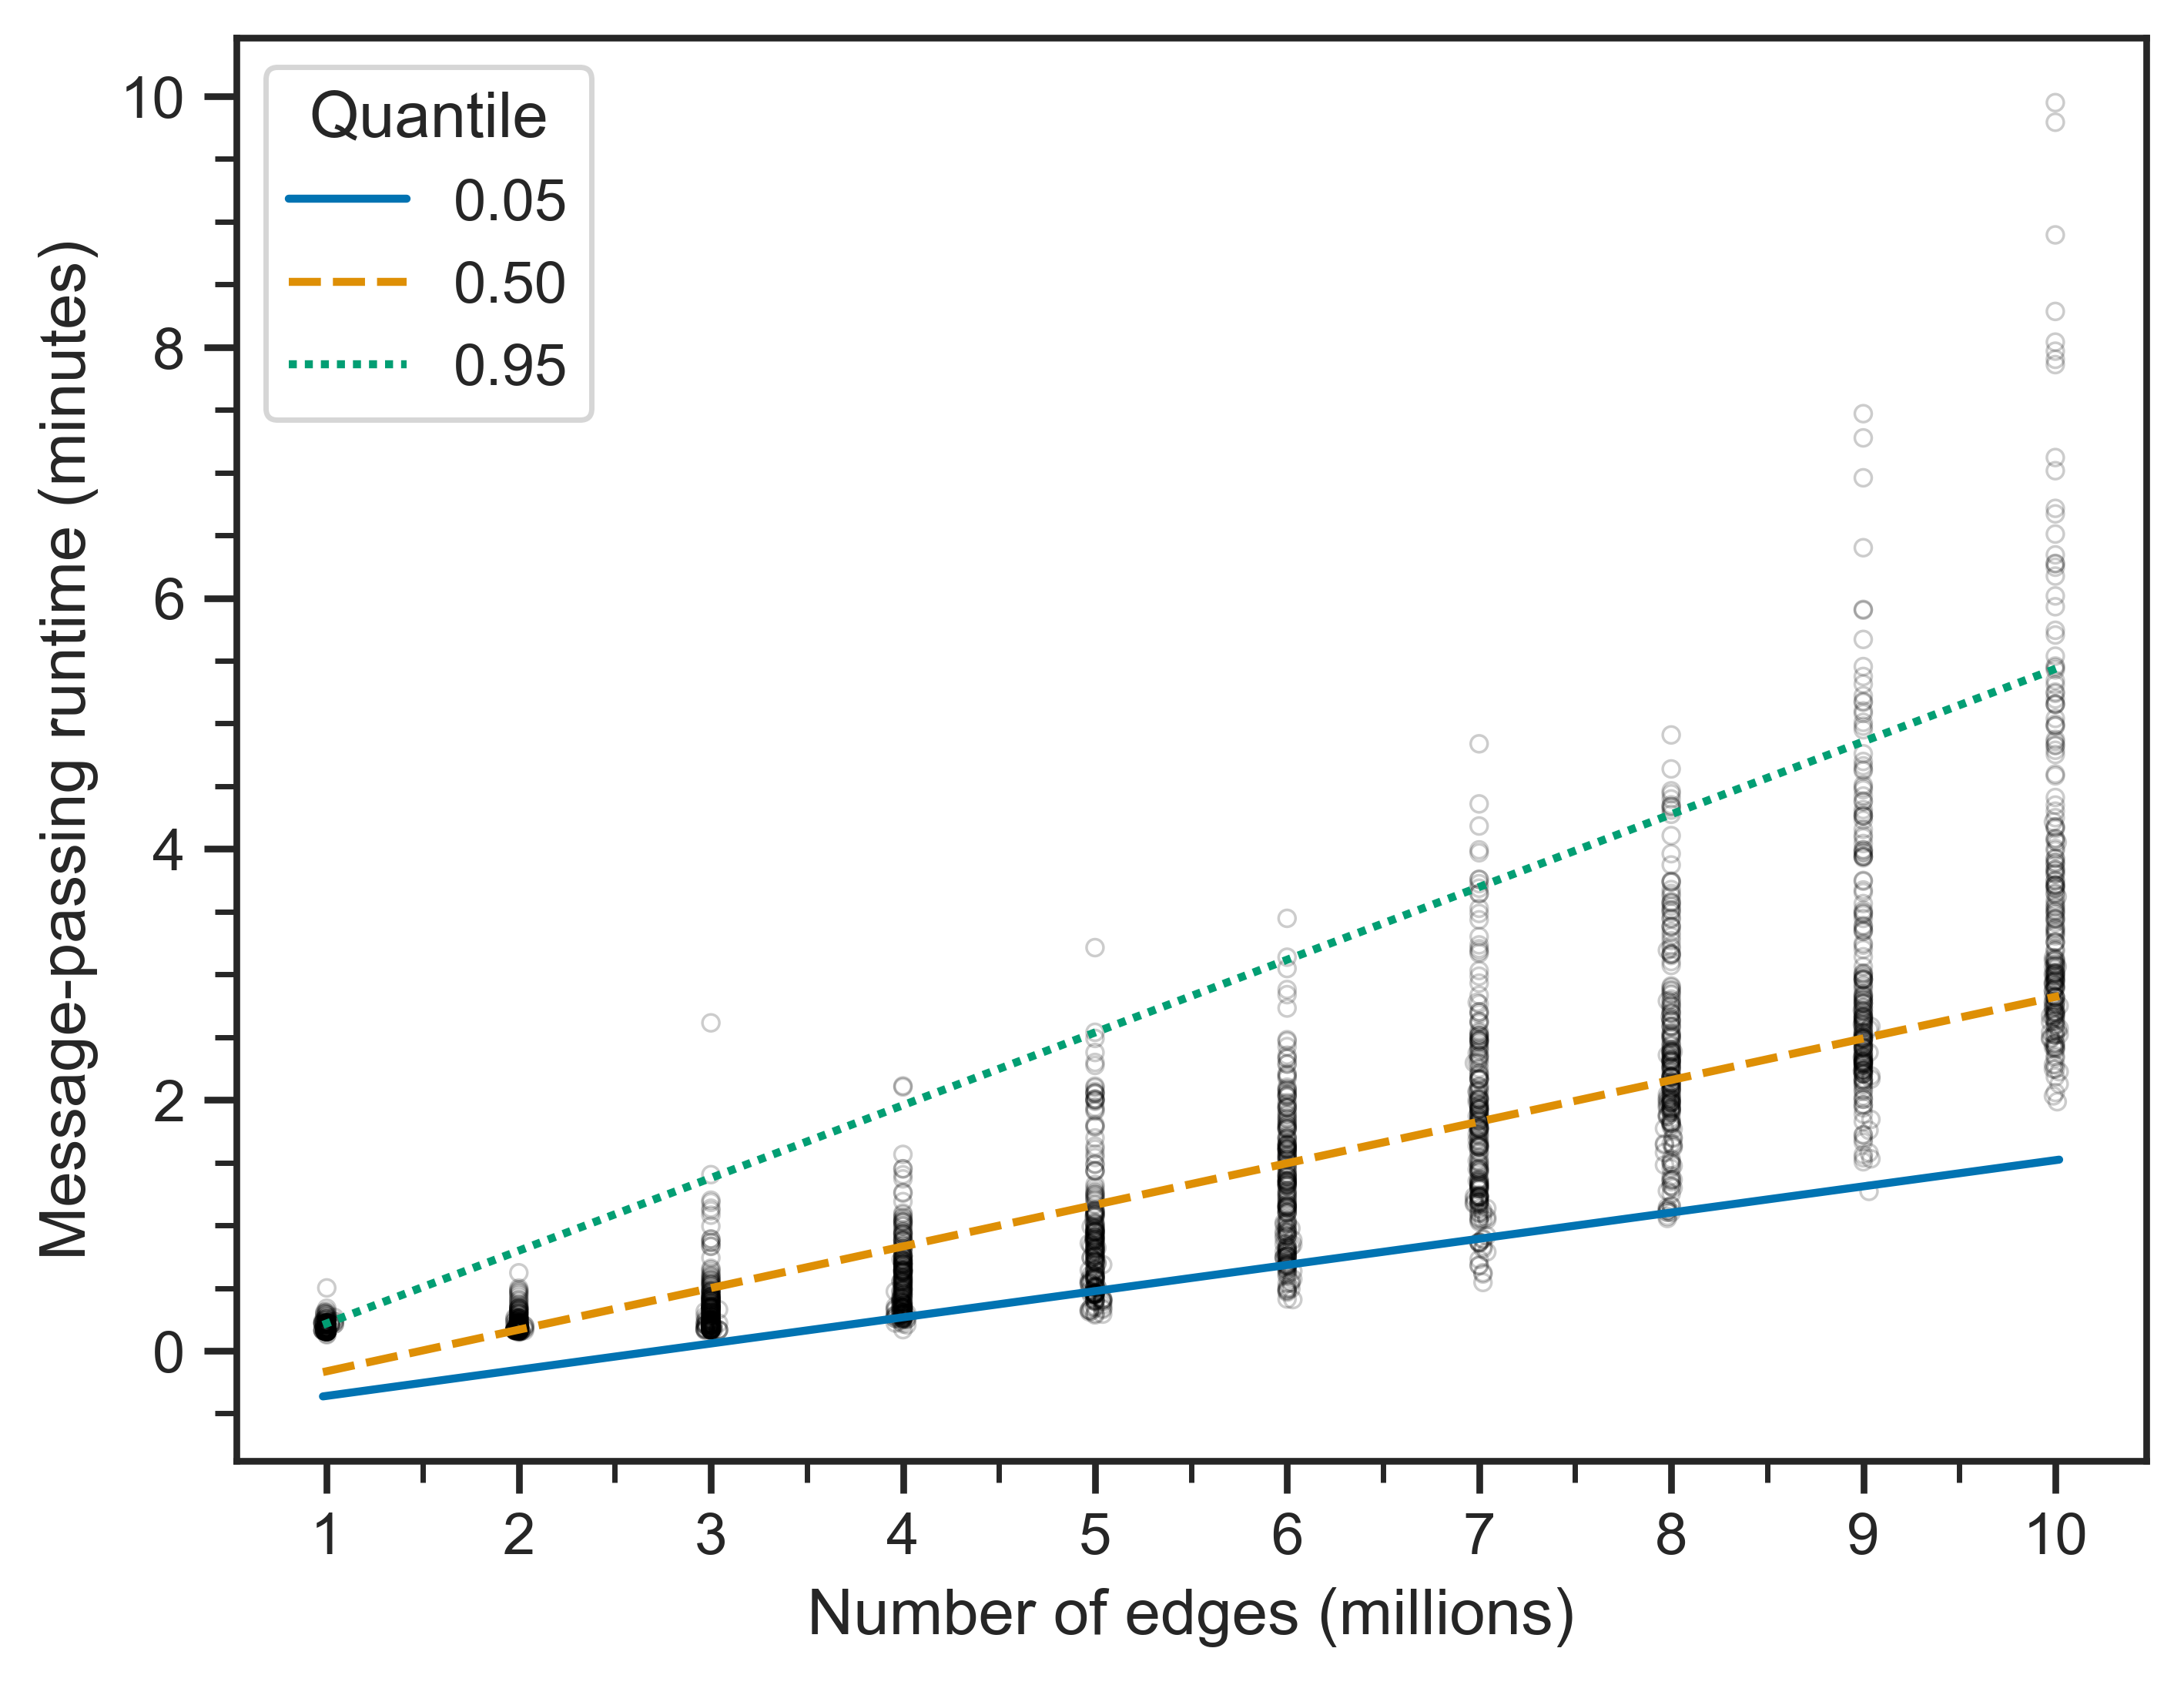
\includegraphics[height=\squareFigHeight]{runtime-regression}
  \caption[Message-passing runtimes with regression lines]{Message-passing runtimes with regression lines.}
\end{figure}
\end{frame}

\end{section}

\begin{section}{Conclusion}

\begin{frame}{Conclusion: Future Work}
  \begin{itemize}
    \item Incorporate differential privacy techniques that are designed for DCT applications that utilize risk scores \citep{Romijnders2024}.
    \item Formally define the security and privacy characteristics of ShareTrace, using the framework proposed by \citet{Kuhn2021} to characterize the latter.
    \item Conduct a simulation-based analysis of asynchronous risk propagation with COVI-AgentSim \citep{Gupta2020}.
    \item Explore the utility and feasibility of integrating decentralized technologies \citep{Benet2014, Troncoso2017, Trautwein2022, Shi2024, Keizer2024} and self-soverign identity \citep{Preukschat2021, Schardong2022} into the system design.
  \end{itemize}
\end{frame}

\end{section}

\begin{section}{Prior Designs and Implementations}

\begin{frame}{Prior Designs and Implementations}
  \begin{itemize}
    \item  ``Thinking like a vertex'' with Apache Giraph
    \item Factor subgraph actors
    \item Driver-monitor-worker framework
    \item Projected subgraph actors \citep{Tatton2022b}
    \item Contact search
  \end{itemize}
\end{frame}

\end{section}

% A section is automatically created for references.
\begin{frame}[allowframebreaks]{References}
  \printbibliography
\end{frame}

\end{document}